%Äquivalenzklassen gibt es schon seit bla bla. Äquivalenzklassen finden jetzt auch in der Informatik Anwendung. bla bla
In diesem Punkt geht es um die Äquivalenzklassen. Sie werden mathematisch beschrieben und danach wird gezeigt, wie sie
in der Informatik Anwendung finden.
\section*{Mathematische Beschreibung der Äquivalenzklassen}
Seien zwei Elemente zu einer Teilmenge R zugeordnet, so spricht man von einer Relation der beiden Elemente und schreibt $\sim$. 
Eine Äquivalenzrelation liegt vor, wenn eine Relation reflexiv, symmetrisch und 
transitiv ist, wie in Abbildung 2.3 dargestellt.
Eine reflexive Relation ist gegeben, wenn jedes Element einer Menge in Relation zu sich selbst steht. %(https://de.wikipedia.org/wiki/Reflexive_Relation, Abruf 14.04.22 14:%$ uhr)
Eine symmetrische Relation ist gegeben, wenn zwei Elemente einer Menge gegeneinander austauschbar sind, wobei die Relation zueinander gegeben bleibt.
%Transitive Relation bedeutet, dass die Relation zweier Elemente auf ein drittes Element übertragbar ist, sofern
Eine transitive Relation ist gegeben, wenn ein Element in Relation zu zwei anderen Elementen steht, so stehen jene beide Elemente auch in Relation zueinander \cite[vgl.][S. 66]{equimaths}.
\begin{figure}[!h]
\centering
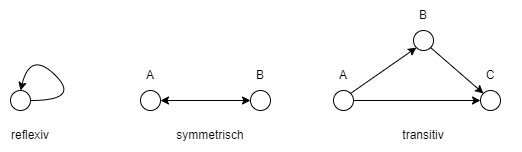
\includegraphics[scale=.9,]{Bilder/EquiDrawio/EigenschaftenEqui.drawio.png}
\caption{Eigenschaften einer Äquivalenzklasse \cite{eigequi1}\cite{eigequi2}}
\end{figure}
\newpage
\paragraph{Definition der Äquivalenzklasse}
$$[a] = \{b \in M ; b \sim a\}$$
\begin{center}
bezeichnet man als Äquivalenzklasse des Elements $a$ in $M$,\\
wobei $\sim$ eine Äquivalenzrelation auf einer Menge $M$ ist und\\
\end{center}
$$a,b \in M.$$
Alle Elemente einer Äquivalenzrelation in der Gesamtheit bezeichnet man als Äquivalenzklasse.
Jedes einzelne Element davon bezeichnet man als Repräsentanten der Äquivalenzklasse \cite[vgl.][S. 66]{equimaths}.

\section*{Äquivalenzklassen in der Informatik}
Um den Bezug zur Informatik herzustellen, wird als Menge der Wertebereich eines Parameters bezeichnet.
Das Prinzip der Äquivalenzklassen kann so auf Parameter angewendet werden, indem ein Parameter in Wertebereiche eingeteilt wird, wie es in Abbildung 2.4 zu sehen ist.
Ein Repräsentant einer Äquivalenzklasse ist ein beliebiger Wert innerhalb des Wertebereichs. 
Es ist gewollt, dass auch Äquivalenzklassen definiert werden, die ein kritisches oder fehlerhaftes Verhalten des Systems erzeugen können.
Wie sie im Detail definiert werden, soll aus dem Requirement hervorgehen.
Sie werden so gewählt, dass sich das System für alle Werte innerhalb der Äquivalenzklasse gleich/ähnlich verhält. Somit reicht es aus, nur 
einen Repräsentanten zu testen. 
Der Sinn der Äquivalenzklassen ist es, dass redundante Testfälle vermieden werden, indem jeweils nur Repräsentanten getestet werden.
Die Anzahl der Testfälle entsteht durch das Produkt aller Äquivalenzklassen pro Parameter. Bei mehreren Parametern sowie der dazugehörigen definierten Wertebereiche
können schnell viele Testfälle entstehen \cite[vgl.][S. 114 ff.]{equiinformatic}.\par
\begin{figure}[h]
\centering
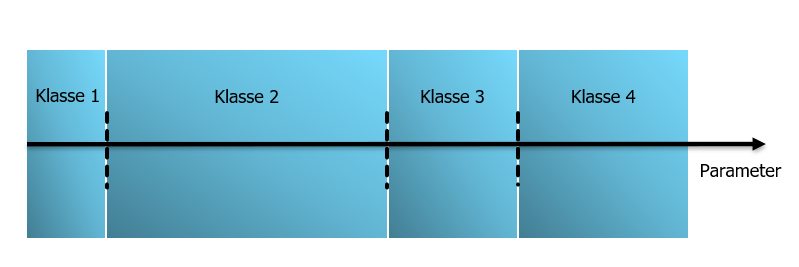
\includegraphics[scale=1.2,]{Bilder/EquiZeitstrahl/ZeitstrahlVerschiedeneKlassenParameter.png} %,6 für VerschieneKlassen
\caption{Einteilung eines Parameters in Äquivalenzklassen \cite[vgl.][S. 114 ff.]{equiinformatic}}
\end{figure}
Möglichkeiten der Testfalleinschränkung \cite[vgl.][S. 120]{equiinformatic}:
\begin{itemize}
\item Testfälle filtern, dass nur oft vorkommende Kombinationen getestet werden
\item Testfälle mit Grenzwerten bevorzugen
\item paarweise Kombination: jeweils zwei Repräsentanten unterschiedler Äquivalenzklassen werden kombiniert
\item Minimalkriterium: jeder Repräsentant ist in mindestens einem Testfall vorhanden
\item Repräsentanten, die ein kritisches/fehlerhaftes Verhalten hervorrufen, werden nicht miteinander kombiniert
\end{itemize}

%Ungültige Äquivalenzklasse bezieht sich darauf, dass es eine Äquivalenzklasse ist, die ein kritisches/fehlerhaftes Verhalten hervorrufen soll.
% (Ausgangskriterium:\\
% ÄK-Überdeckung = ( getestete ÄK / alle ÄK ) x 100\%) \cite[S.114 ff.]{equiinformatic}







































% (
% "
% Sicherstellen, dass jeder Repräsentant einer Äquivalenzklasse mit
% jedem Repräsentanten der anderen Äquivalenzklassen in einem
% Testfall zur Ausführung kommt (d. h. paarweise Kombination
% statt vollständiger Kombination)."
% Verbesserung:
% "Als Minimalkriterium sicherstellen, dass jeder Repräsentant einer
% Äquivalenzklasse in mindestens einem Testfall vorkommt."

% "Es werden allerdings nur einzelne Ein- oder Ausgabebedingungen
% betrachtet, mögliche Abhängigkeiten oder Wechselwirkungen zwischen
% den Bedingungen werden nicht berücksichtigt bzw. sind sehr
% aufwendig zu berücksichtigen (durch weitere Aufteilung der Äquivalenzklassen
% und entsprechende Kombinationen)."
% )

% reflexiv:\\
% 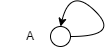
\includegraphics[scale=.9,]{Bilder/EquiDrawio/reflexiv.drawio.png}
% symmetrisch:\\
% 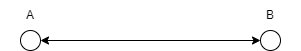
\includegraphics[scale=.9,]{Bilder/EquiDrawio/symmetrisch.drawio.png}
% transitiv:\\
% 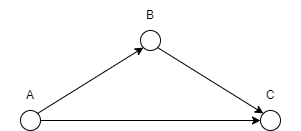
\includegraphics[scale=.9,]{Bilder/EquiDrawio/transitiv.drawio.png}
% \textbf{Bildinfo 3 Bilder reflexiv etc: 3 Eigenschaften von Äquivalenzklassen}

% \begin{figure}[!h]
% \centering
% 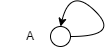
\includegraphics[scale=.9,]{Bilder/EquiDrawio/reflexiv.drawio.png}
% \caption{reflexiv}
% \end{figure}

% \begin{figure}[!h]
% \centering
% 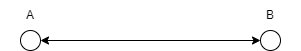
\includegraphics[scale=.9,]{Bilder/EquiDrawio/symmetrisch.drawio.png}
% \caption{symmetrisch}
% \end{figure}

% \begin{figure}[!h]
% \centering
% 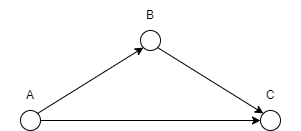
\includegraphics[scale=.9,]{Bilder/EquiDrawio/transitiv.drawio.png}
% \caption{transitiv}
% \end{figure}